\section{Numerical approach and results}
\subsection{Numerical implementation}
In order to find Nash equilibria and fix-points of the behaviorally modified Rosenzweig-MacArthur  system \Cref{sec:model_rm}, we use the formulation of \Cref{eq:comp_form}. We discretize space uniformly, using the trapezoidal rule to evaluate the integrals. By using the trapezoidal rule, we keep a banded sparsity pattern in the coupling of the locations. The equations \Cref{eq:dynamics} and the derivatives of the monomorphic payoffs \Cref{eq:mon_eq_forms} are formulated via. the symbolic language CasADi \citep{Andersson2019}, where we then solve the complementarity problem as a feasibility problem using IPOPT \citep{wachter2006implementation} using the HSL subroutines for linear algebra \citep{hsl2007collection}. We checked the numerics by also solving the problem with non-linear complementarity routine from the open-source package SICONOS \citep{acary2019introduction}.

The numerical approach for finding Nash equilibria and fixed points is extremely fast, and should scale to much larger problems. It allows for determination of fixed-points of the dynamics in less than 1 second with several hundred grid points. Simulating the population dynamics is, in contrast, a comparatively slow affair since we simulate the population dynamics using a forward Euler method.

\subsection{Population dynamics and levels}
% on model introduced in \Cref{sec:model_rm}.
With a numerical approach in place, we can study the population dynamics and the sensitivity of \Cref{sec:model_rm} to parameters. We vary the carrying capacity $(K)$ and the intraspecific predator competition $(c)$. We are interested in both  the population levels at equilibrium, and the associated spatial distributions.
The parameters for the model are: \\
\begin{tabular}{l l l}
  Name & Value & Meaning \\
  $q$ & 3 & Refuge quality \\
  $K_0$ & $10^{-4}$ & Minimal carrying capacity \\
  $\beta_{p,0}$ & $10^{-4}$ & Minimal predator clearance rate \\
  $\beta_c$ & 1 & Consumer clearance rate \\
  $\mu_p$ & 0.15 & Predator metabolic rate \\
  $F_p$ & 100 & Predator maximum growth rate \\
  $\epsilon$ & 0.1 & Trophic efficiency
\end{tabular}
\\
\begin{figure}[H]
  \caption{Phase portrait of the population dynamics of the behaviorally modified Rosenzweig-MacArthur system at carrying capacity of $K=40$. The blue line illustrates a system trajectory with initial conditions $C(0)=8,~P(0)=8$.}
  \label{fig:dynamics}
  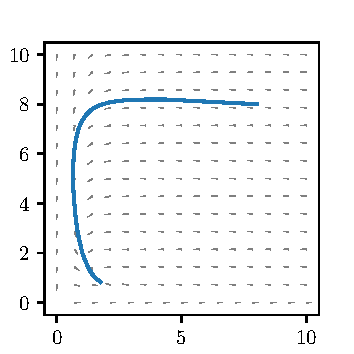
\includegraphics{plots/dynamics.pdf}
\end{figure}
\Cref{fig:dynamics} illustrates the phase portrait for the behaviorally modified Rosenzweig-MacArthur model, along with a sample trajectory. The direction of the flow is consistent with the usual Rosenzweig-MacArthur model. The phase portrait reveals that the system dynamics have been stabilized. Looking at the sample trajectory, this stabilization is quite substantial with not even a full oscillation. The stable dynamics stand in contrast to the Rosenzweig-MacArthur model with constant behavior $(\sigma_p=\sigma_c=1)$ where the point of the Hopf bifurcation has been passed, leading to limit cycles. Adding optimal individual behavior appears to eliminate the paradox of enrichment \citep{rosenzweig1971paradox}, which is a common consequence of optimal behavior \citep{abrams2010implications}.
\begin{figure}[H]
  \caption{Panel $(A)$ shows population levels of consumers (blue) and predators (red) at equilibrium with changing carrying capacity $(K)$. Panel $(B)$ again shows the population levels, but with varying intraspecific predator competition $(C)$.}
  \label{fig:pop_levels}
  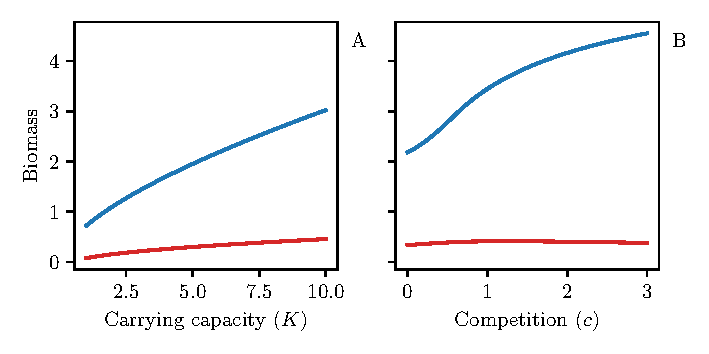
\includegraphics{plots/pop_levels_c.pdf}
\end{figure}
\Cref{fig:pop_levels} reveals how the population levels of consumers and predators change at equilibrium with varying refuge quality (\Cref{fig:pop_levels}(A)), carrying capacity (\Cref{fig:pop_levels}(B)) and intraspecific predator competition (\Cref{fig:pop_levels}(C)).
Increasing the quality of the refuge (\Cref{fig:pop_levels})(A) initially causes an increase in consumer populations (\Cref{fig:pop_levels}(A, blue)) and a decrease in predator populations.

A higher carrying capacity causes higher populations of both consumers and predators populations at equilibrium (\Cref{fig:pop_levels}). The increase in both populations is probably because the behavioral choice allows the consumers to avoid the risk of predation, while achieving the same fitness.

Varying the intraspecific predator competition causes an increase in the population of predators (\Cref{fig:pop_levels}(C, red)) until a point where the population stabilizes (\Cref{fig:pop_levels}($c\approx 1/3$)), a modified hydra phenomenon \citep{abrams2009does}. The population of consumers continues to increase (\Cref{fig:pop_levels}(C, blue)), corresponding to expectations \citep{abrams1992predators}.


\subsubsection{Spatial distribution}
\begin{figure}[H]
  \caption{Spatial distribution of consumers $(A)$ and predators $(B)$ at the equilibrium with increasing carrying capacity $(K)$.}
  \label{fig:strat_car}
  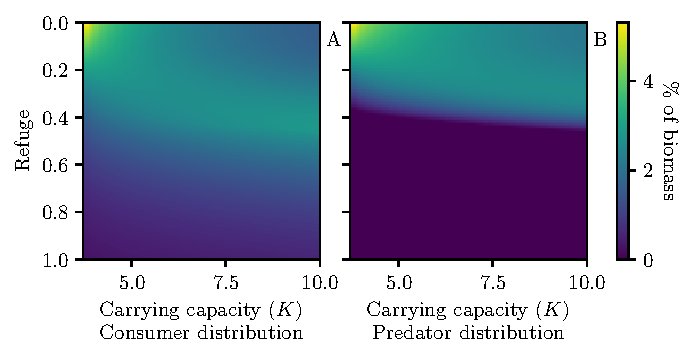
\includegraphics{plots/increasing_car_cap_c.pdf}
\end{figure}
The plots in (\Cref{fig:strat_car}) illustrate the strategies of the consumers (\Cref{fig:strat_car}(A)) and predators (\Cref{fig:strat_car}) at equilibrium when carrying capacity varies. At low carrying capacities, both consumers and predators are relatively spread out, with the peak concentration about halfway to the refuge. As the carrying capacity increases, the distribution becomes more concentrated and clusters closer to the refuge. The increase in concentration is most marked for the predators. Predators are almost uniformly distributed in the space 0.5-1 at low carrying capacity, while the majority forms a cluster just above the consumer layer at a carrying capacity of 7. Thus the gain from clustering gradually outweighs the loss from the intraspecific predator competition. That both predator and consumer population increase must be the driving factor behind the peak population concentration moving to less productive areas.

A higher carrying capacity leads to more concentrated populations, but the increase in populations leads to greater risk-aversion from the consumers so they concentrate in less desirable zones.

\begin{figure}[H]
  \caption{Distribution of consumers $(A)$ and predators $(B)$ at equilibrium under changing predator competition $(c)$.}
  \label{fig:strat_comp}
    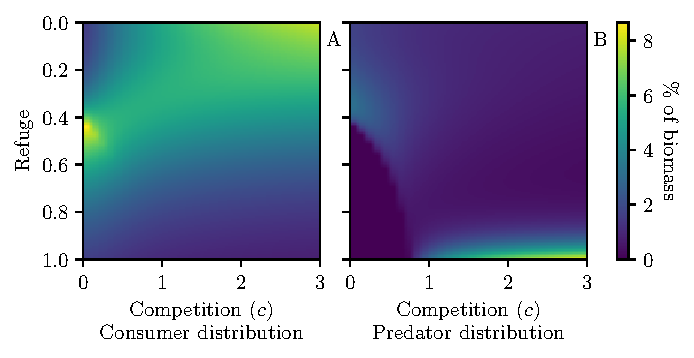
\includegraphics{plots/increasing_competition_c.pdf}
\end{figure}
In \Cref{fig:strat_comp} the intraspecific predator competition is varied and we see the emergent  equilibrium strategy of the consumers (\Cref{fig:strat_comp}(A)) and predators (\Cref{fig:strat_comp}(B)). When there is no intraspecific predator competition, both consumers and predators are highly concentrated at about 0.4. The equilibrium distribution of predators spreads out as we increase the intraspecific predator competition. The previous equilibrium becomes unstable, since the gain from clustering on the consumers is outweighed by the risk of encountering other predators. As the predators gradually spread and go the safest zone (1), it is echoed by the consumers spreading out and going to the most productive area (0) as well, further incentivicizing predator-spread. The spreading out of the consumer population can be interpreted in terms of the ideal free distribution. An increase in consumer population \Cref{fig:pop_levels} causes an increase in concentration on the less productive spots. When the consumer population spreads out, the distribution trends towards the more productive layers.

\begin{comment}
\begin{figure}[H]
  \caption{Consumer (A) and predator (B) concentration at equilibrium as a function of changing refuge quality}
  \label{fig:ref_qual}

    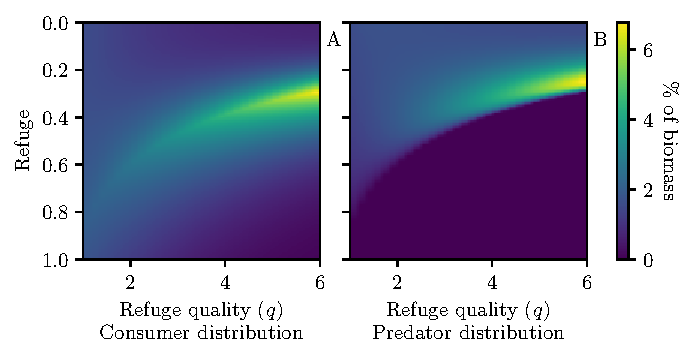
\includegraphics{plots/increasing_refuge_quality_c.pdf}
\end{figure}
\Cref{fig:ref_qual} shows the strategy of consumers (\Cref{fig:ref_qual}(A)) and predators (\Cref{fig:ref_qual}(B)) at equilibrium with varying refuge quality.
\end{comment}
